% % % % % % % % % % % % % % % % % % % % % % % % % % % % % % % % % % % % % % % % % % % %
%                                                                                     %
% Short Sectioned Assignment LaTeX Template Version 1.0 (5/5/12)                      %
% This template has been downloaded from: http://www.LaTeXTemplates.com               %
%                                                                                     %
% Original author:  Frits Wenneker (http://www.howtotex.com)                          %
%                                                                                     %
% Modified by: Fco Javier Sueza Rodríguez (fcosueza@disroot.org)                      %
%                                                                                     %
% Changes:                                                                            %
%	    - Custom Chapters, Sections and Subsections (titlesec package)                %
%           - Document type scrbook (oneside)                                         %
%           - Use babel-lang-spanish package and marvosym                             %
%           - Use hyperref, enumitem, tcolorbox and glossaries packages               %
%           - Use Time New Roman (mathptmx), Helvetic and Courier fonts               %
%                                                                                     %
% License: CC BY-NC-SA 3.0 (http://creativecommons.org/licenses/by-nc-sa/3.0/)        %
%                                                                                     %
% % % % % % % % % % % % % % % % % % % % % % % % % % % % % % % % % % % % % % % % % % % %

%-----------------------------------------------%
%	              Packages                  %
%-----------------------------------------------%

\documentclass[paper=a4, fontsize=11pt, oneside]{scrbook}

% ---- Text Input/Output ----- %

\usepackage[T1]{fontenc}
\usepackage[utf8]{inputenc}
\usepackage{mathptmx}
\usepackage[scaled=.92]{helvet}
\usepackage{courier}
\usepackage[indent=12pt]{parskip}

\usepackage{geometry}
\geometry{verbose,tmargin=3cm,bmargin=3cm,lmargin=2.6cm,rmargin=2.6cm}

% ---- Language ----- %

\usepackage[spanish]{babel}
\usepackage{marvosym}

% ---- Another packages ---- %

\usepackage{amsmath,amsfonts,amsthm}
\usepackage{graphics,graphicx}
\usepackage{titlesec}
\usepackage{fancyhdr}
\usepackage{tcolorbox}
\usepackage{hyperref}
\usepackage{enumitem}
\usepackage[automake]{glossaries}

%--------------------------------------------------------------------%
%                      Customizing Document                          %
%--------------------------------------------------------------------%


% ----------- Custom Chapters, Sections and Subsections -------------- %

\titleformat{\chapter}[display]
			{\bfseries\Huge}
			{Tema \ \thechapter} {0.5ex}
			{\vspace{1ex}\centering}

\titleformat{\section}[hang]
			{\bfseries\Large}
			{\thesection}{0.5em}{}

\titleformat{\subsection}[hang]
			{\bfseries\large}
			{\thesubsection}{0.5em}{}

\titleformat{\subsubsection}[hang]
			{\bfseries\large}
			{\thesubsubsection}{0.5em}{}

\hypersetup{
    colorlinks=true,
    linkcolor=black,
    urlcolor=magenta
}

% ------------------- Custom heaaders and footers ------------------- %

\pagestyle{fancyplain}

\fancyhead[]{}
\fancyfoot[L]{}
\fancyfoot[C]{}
\fancyfoot[R]{\thepage}

\renewcommand{\headrulewidth}{0pt} % Remove header underlines
\renewcommand{\footrulewidth}{0pt} % Remove footer underlines

\setlength{\headheight}{13.6pt} % Customize the height of the header

% --------- Numbering equations, figures and tables ----------------- %

\numberwithin{equation}{section} % Number equations within sections
\numberwithin{figure}{section} % Number figures within sections
\numberwithin{table}{section} % Number tables within sections

% ------------------------ New Commands ----------------------------- %

\newcommand{\horrule}[1]{\rule{\linewidth}{#1}} % Create horizontal rule command


%----------------------------------------------------------------------------------------
%	TÍTULO Y DATOS DEL ALUMNO
%----------------------------------------------------------------------------------------

\title{
\vspace{10ex}
\normalfont \normalsize
\Huge \textbf{Tarea 7: Instalación y Configuración de Ubuntu Desktop 22.04 LTS}
}
\author{Francisco Javier Sueza Rodríguez}
\date{\normalsize\today}

%----------------------------------------------------------------------------------------
%                                     DOCUMENTO
%----------------------------------------------------------------------------------------
\begin{document}

\maketitle

\thispagestyle{empty}

\vspace{68ex}

\begin{center}
    \begin{tabular}{l l}
        \textbf{Centro}: & IES Aguadulce \\
        \textbf{Ciclo Formativo}: & Desarrollo Aplicaciones Web (Distancia)\\
        \textbf{Asignatura}: & Sistemas Informáticos\\
        \textbf{Tema}: & Tema 7 -  Instalación y Configuración de Linux\\
    \end{tabular}
\end{center}

\newpage

\tableofcontents

\newpage

\listoffigures

\newpage

\section{Caso Práctico}
Uno de los directivos de la empresa ha solicitado a Ada la puesta en marcha de un sistema operativo GNU/LINUX en su equipo y ésta traslada la petición a Antonio para que lo haga conjuntamente con Juan. Ellos fueron los que instalaron en los equipos Windows 10 y Windows 8.1, y ahora instalarán el nuevo sistema operativo en una partición libre que dejaron en su momento, precisamente porque pensaron que en un futuro podrían recibir peticiones de este tipo.

\section{Actividades}
\subsection{Actividad 1: Un poco de documentación}
\subsubsection{Enunciado}
Indica lo que permiten o no permiten las siguientes licencias de derechos de autor Creative Commons. Rellena la siguiente tabla atendiendo al ejemplo de la primera fila.

\begin{figure}[H]
    \centering
    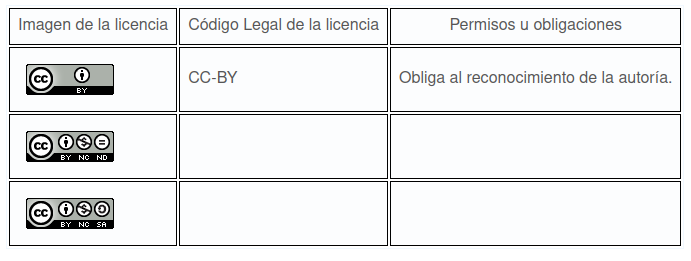
\includegraphics[scale=0.60]{tabla-cc.png}
    \caption{Tabla de licencias Creative Commons}
\end{figure}

Responde a las siguientes preguntas:

\begin{enumerate}[label=\alph*.]
    \item ¿Cuál es el principal objetivo de la licencia GNU GPL?
    \item ¿Qué podemos hacer con un software cuya licencia cumpla la libertad 3?
    \item Si tengo un software cuya licencia cumple la libertad 1: ¿Podemos distribuir copias? Razona la respuesta.
\end{enumerate}

\subsubsection{Solución}
En primer lugar, vamos a rellenar la tabla sobre las licencias Creative Commons especificando el código legal de cada una y sus permisos u obligaciones.

En la siguiente figura, se muestra la tabla completada.

\begin{figure}[H]
    \centering
    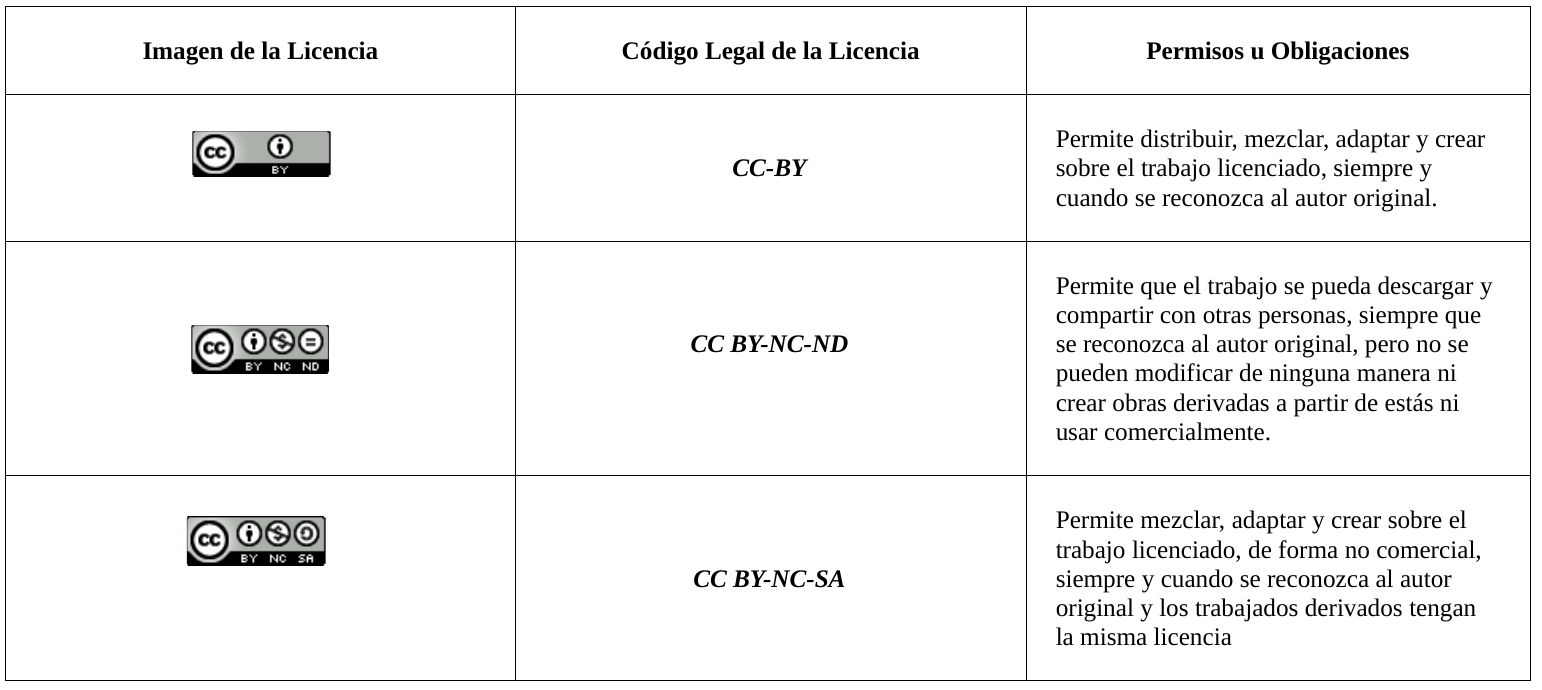
\includegraphics[scale=0.40]{tabla-cc-completa.png}
    \caption{Tabla licencias Creative Commons - Completada}
\end{figure}

A continuación, vamos a \textbf{responder a las preguntas} planteadas sobre la licencia GPL:

\begin{enumerate}[label=\alph*.]
    \item El \textbf{principal objetivo} de la licencia GPL es el de garantizar la libertad para modificar y compartir el software que se encuentre bajo dicha licencia y sus derivados.

    \item Con un software cuya licencia cumpla la \textbf{libertad 3}, podremos realizar todas las \textbf{modificaciones} que consideremos oportunas en dicho software y \textbf{redistribuirlo}.

    \item Si tenemos un software que cuya licencia \textbf{sólo} cumple la \textbf{libertad 1} no tenemos permisos para redistribuirlo, ya que esta libertad solo otorga permisos para \textbf{adaptarlo a nuestra necesidades} y \textbf{estudiar su funcionamiento}, quedando excluido en este punto la redistribución.

    Para que el software se pudiera redistribuir libremente debería cumplir la \textbf{libertad 3}.
\end{enumerate}

\subsection{Actividad 2: Instalación de Ubuntu}

\textbf{¡IMPORTANTE!} Si estás utilizando Oracle VirtualBox como software de virtualización para estas tareas, es posible que cuando instales Ubuntu 22.04 y lo inicies no veas nada en la pantalla (pantalla negra). Para evitar/arreglar esto, con la VM apagada prueba a cambiar en su configuración lo siguiente: ``Configuración > Pantalla > Controlador gráfico: VMSVGA''

\subsubsection{Enunciado}
Instala la versión 22.04 LTS del sistema operativo Ubuntu (versión Desktop) en la partición libre que dejaste en la máquina virtual de la tarea 4. Esta versión está disponible sólo para sistemas de 64 bits, en caso de tener que instalar una versión para 32 bits lee las indicaciones del apartado 2.- Información de interés. Es muy importante recordar que se deben mantener las instalaciones de Windows de las tareas previas.

Si no realizaste la tarea 4, para que ésta sea válida tienes que instalar Ubuntu Desktop 22.04 LTS junto con Windows 10 en una máquina virtual definida con un tamaño de disco duro de 70 GB y con dos particiones de 35 GB, una para cada sistema. En ese caso primero debes instalar Windows 10 y luego Ubuntu Desktop  22.04 LTS.

Durante la instalación de Ubuntu debes definir un usuario local cuyo nombre de usuario sea la primera letra de tu nombre seguido de tus apellidos completos, por ejemplo, para \textbf{José Luis Pérez Puertas} el usuario debería ser \textbf{jlperezpuertas}. Respecto a la clave de este usuario ponle \textbf{admin2223}.

\textbf{Capturas}:
\begin{itemize}
    \item Elección del archivo de instalación del sistema.
    \item Inicio del proceso de instalación.
    \item Actualizaciones y otro software. Justifica las opciones elegidas.
    \item Tipo de instalación: ``Instalar Ubuntu junto a Windows 10'', ``Borrar disco e instalar Ubuntu''' o ``Más opciones''. Justifica tu elección.
    \item Creación del usuario y establecimiento de la contraseña.
    \item Muestra de que el sistema ha sido debidamente instalado.
\end{itemize}

\subsubsection{Solución}
En este ejercicio vamos a realizar la instalación de \textbf{Ubuntu 22.04 LTS} (\textbf{Jammy Jellyfish}), la última versión estable de la distribución de Canonical lanzada en Abril de 2022.

Para realizar la instalación, vamos a llevar a cabo una \textbf{serie de pasos} que enumeraremos a continuación, ilustrándolos con las capturas de pantalla pedidas de forma que el proceso se entienda más claramente.

\begin{enumerate}
    \item En primer lugar, vamos a descargar la imagen ISO de \textbf{Ubuntu 22.04 LTS}, en concreto, su versión para \textbf{AMD64} que podemos encontrar en \href{https://releases.ubuntu.com/jammy/}{este enlace}.

    \begin{figure}[H]
        \centering
        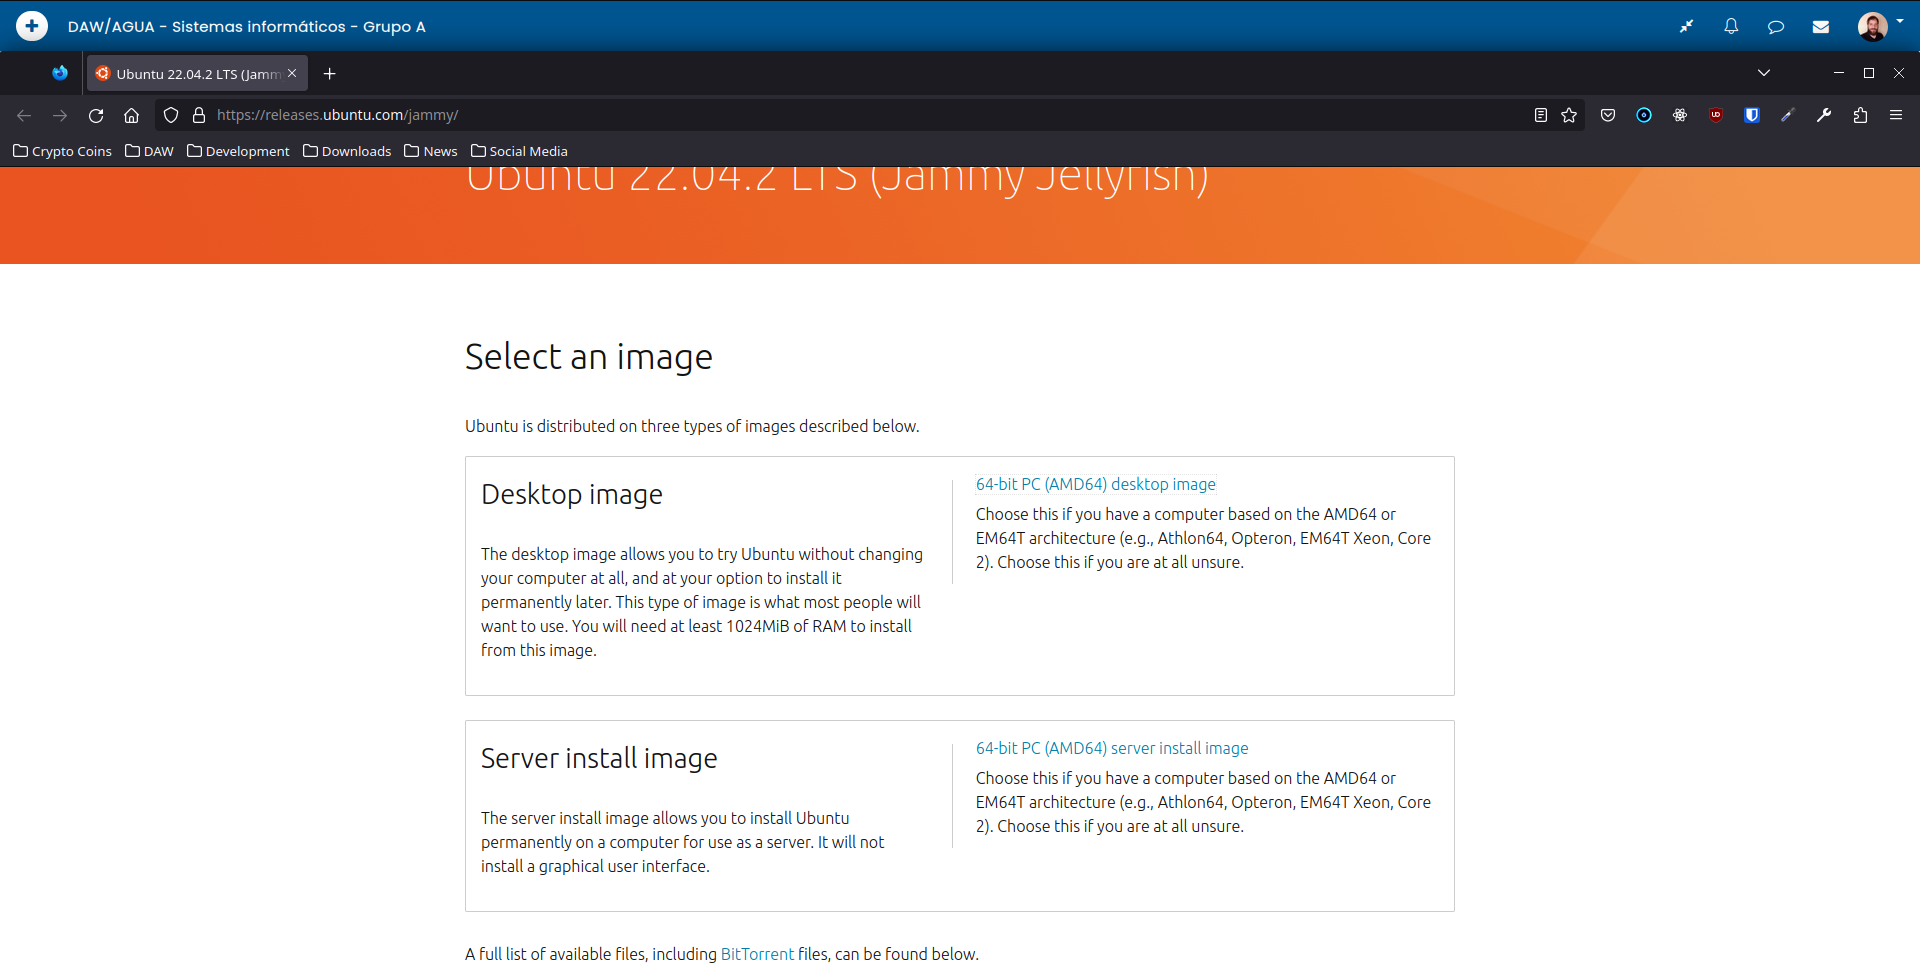
\includegraphics[scale=0.25]{ubuntu-install-1.png}
        \caption{Descarga de la imagen de Ubuntu 22.04 LTS}
    \end{figure}

    \item Una vez descargada la imagen ISO, debemos \textbf{cargar la imagen en VMWare}. Para ello, iniciamos VMWare y pulsamos con el botón derecho sobre nuestra máquina virtual y seleccionamos la opción ``\textit{\textbf{Virtual Machine Setting}}''. En la ventana que se nos muestra, seleccionamos la opción ``\textit{\textbf{CD/DVD SATA}}'', lo que nos mostrará otra ventana donde, seleccionando la opción ``\textit{\textbf{Use ISO image}}'', nos permitirá seleccionar nuestra imagen ISO, como podemos ver en la siguiente captura.

    \begin{figure}[H]
        \centering
        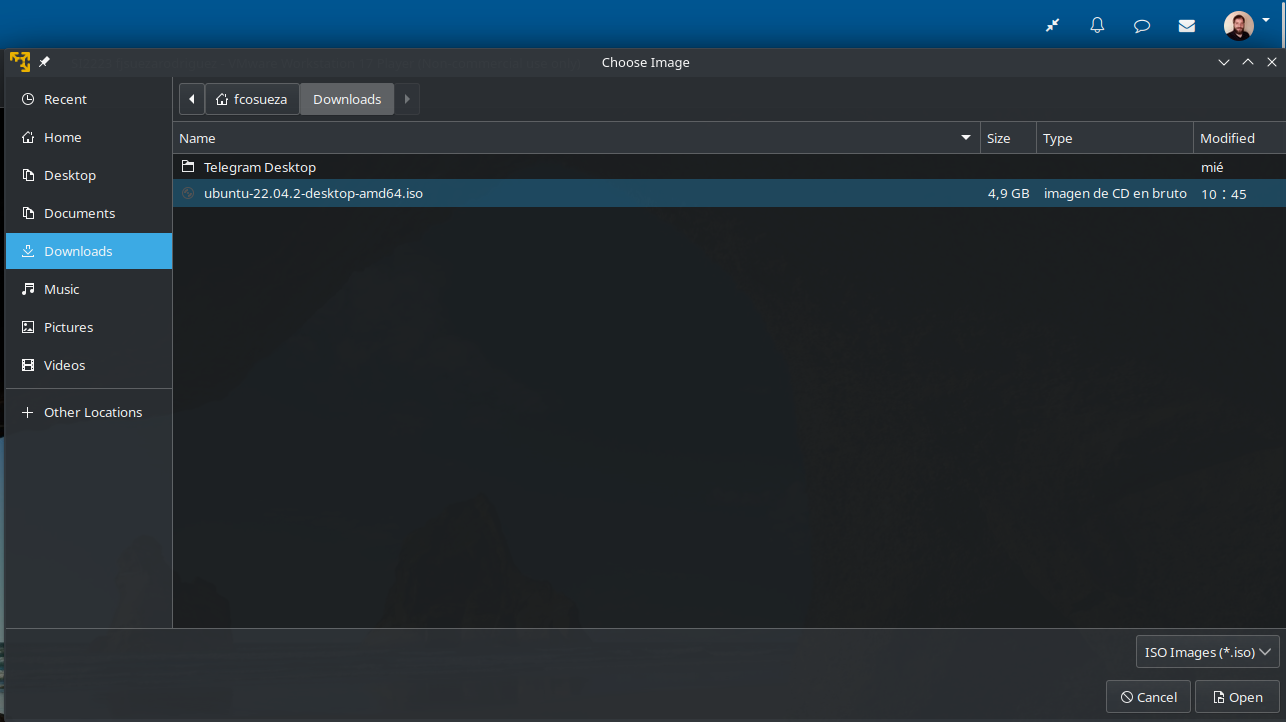
\includegraphics[scale=0.35]{ubuntu-install-2.png}
        \caption{Selección de imagen ISO en VMWare}
    \end{figure}

    \item Tras iniciar la imagen ISO, nos aparecerá la ventana de \textbf{GRUB}, donde podremos seleccionar diferentes opciones, teniendo que elegir la opción ``\textbf{Try or Install Ubuntu}''. Una vez seleccionada, se nos mostrará el asistente para comenzar el inicio de la instalación.

    \begin{figure}[H]
        \centering
        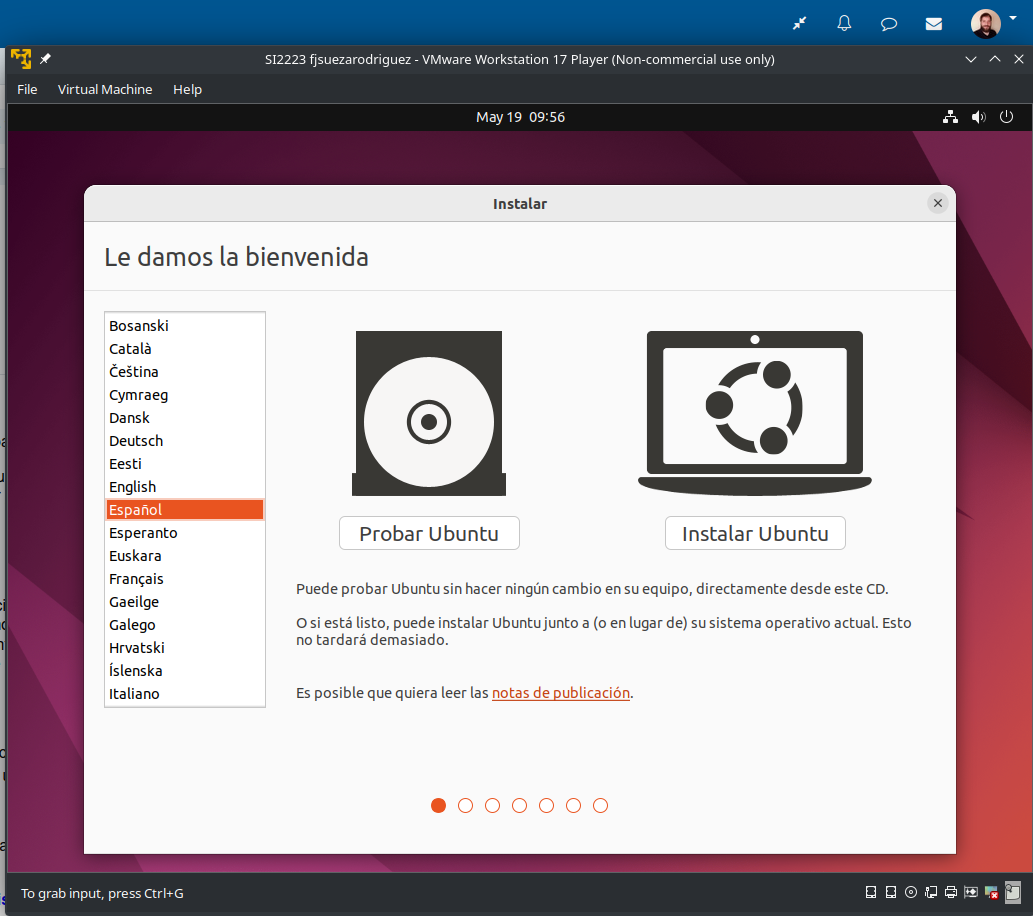
\includegraphics[scale=0.45]{ubuntu-install-3.png}
        \caption{Asistente de instalación de Ubuntu}
    \end{figure}

    En esta ventana, podemos seleccionar el idioma y si queremos probar o instalar Ubuntu. Nosotros hemos seleccionado
    el idioma \textbf{Español} y la opción \textbf{Instalar Ubuntu}.


    \item La siguiente pantalla, nos mostrará opciones para seleccionar la \textbf{distribución} del teclado, nosotros seleccionaremos la opción \textbf{Spanish} en ambos cuadros de opciones. También tenemos la opción ``\textbf{Detectar la distribución del teclado}, que nos pedirá que pulsemos diferentes caracteres en nuestro teclado para realizar la detección y nos sugerirá la opción de distribución más adecuada para nuestro teclado. Pulsamos en \textbf{continuar}.

    \begin{figure}[H]
        \centering
        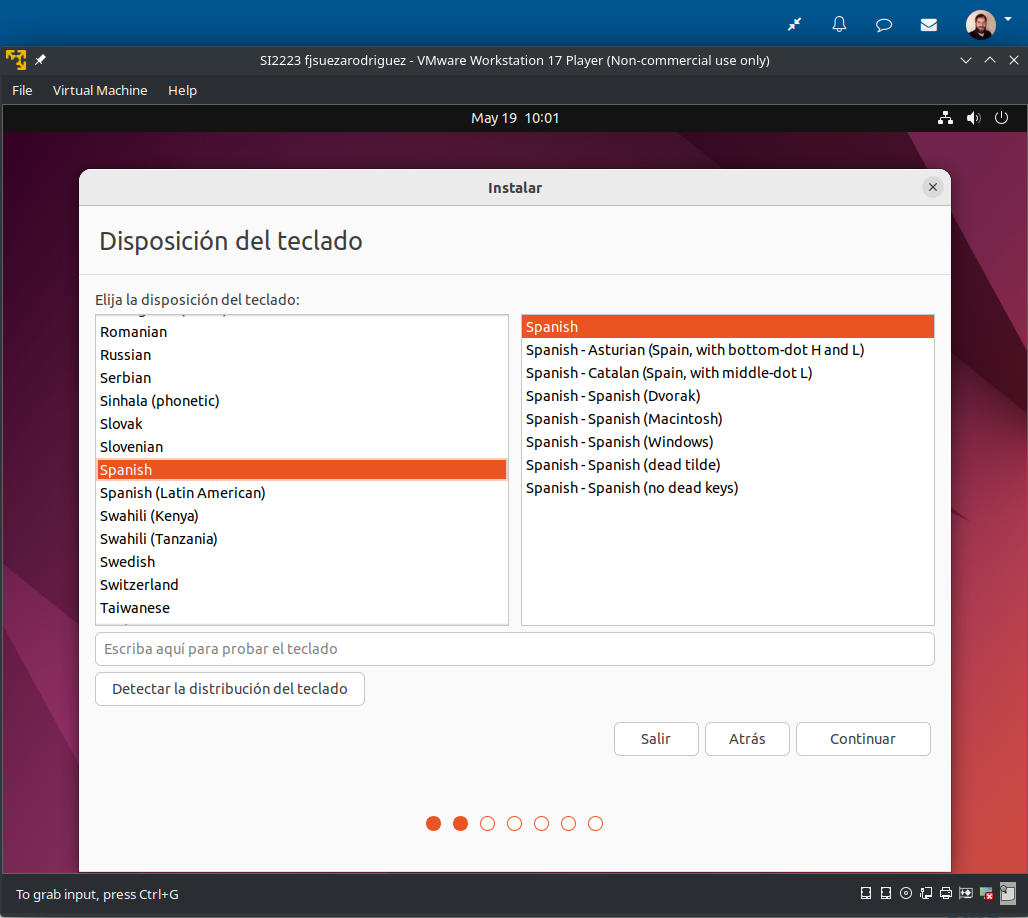
\includegraphics[scale=0.45]{ubuntu-install-4.png}
        \caption{Selección de la distribución del teclado}
    \end{figure}

    \item La siguiente pantalla que nos muestra el instalador es la de \textbf{Actualizaciones y Otro Software}. Aquí se nos ofrecen opciones sobre el tipo de instalación que se va a realizar, así como si se bajaran actualizaciones durante el proceso o se instalarán software de terceros. En la siguiente captura vemos esta pantalla y las opciones que hemos seleccionado.

    Por un lado, hemos seleccionado la opción \textbf{Instalación normal}, ya que esto nos instala todos los paquetes de software, además de los básicos, como pueden ser paquetes ofimáticos, reproductores multimedia, etc..

    También hemos seleccionado la opción \textbf{Descargar actualizaciones...}, para que durante el proceso de instalación se actualicen los paquetes que sean necesarios. Esto es una buena idea, ya que si no lo hacemos durante el proceso de instalación, tendríamos que hacerlo al acabar ésta. Así, se realizarán los dos procesos la vez, asegurándonos de que contamos con las \textbf{últimas versiones} del software instalado, las cuales pueden tener solo mejoras de funcionalidad, pero también puede ser que solución problemas de seguridad en las diferentes aplicaciones.

    Por último, hemos seleccionado también la opción \textbf{Instalar software de terceros...}. Esta opción es importante que la marquemos, aunque ciertamente no siempre es necesaria, pero hay ciertos dispositivos, como tarjetas wifi o adaptadores gráficos, que pueden requerir de la instalación de drivers desarrollados por terceros, en muchos casos de la propia compañía que produce el hardware, para su correcto funcionamiento y desempeño.

    En la siguiente captura, vemos esta pantalla con todas las opciones que hemos seleccionado.

    \begin{figure}[H]
        \centering
        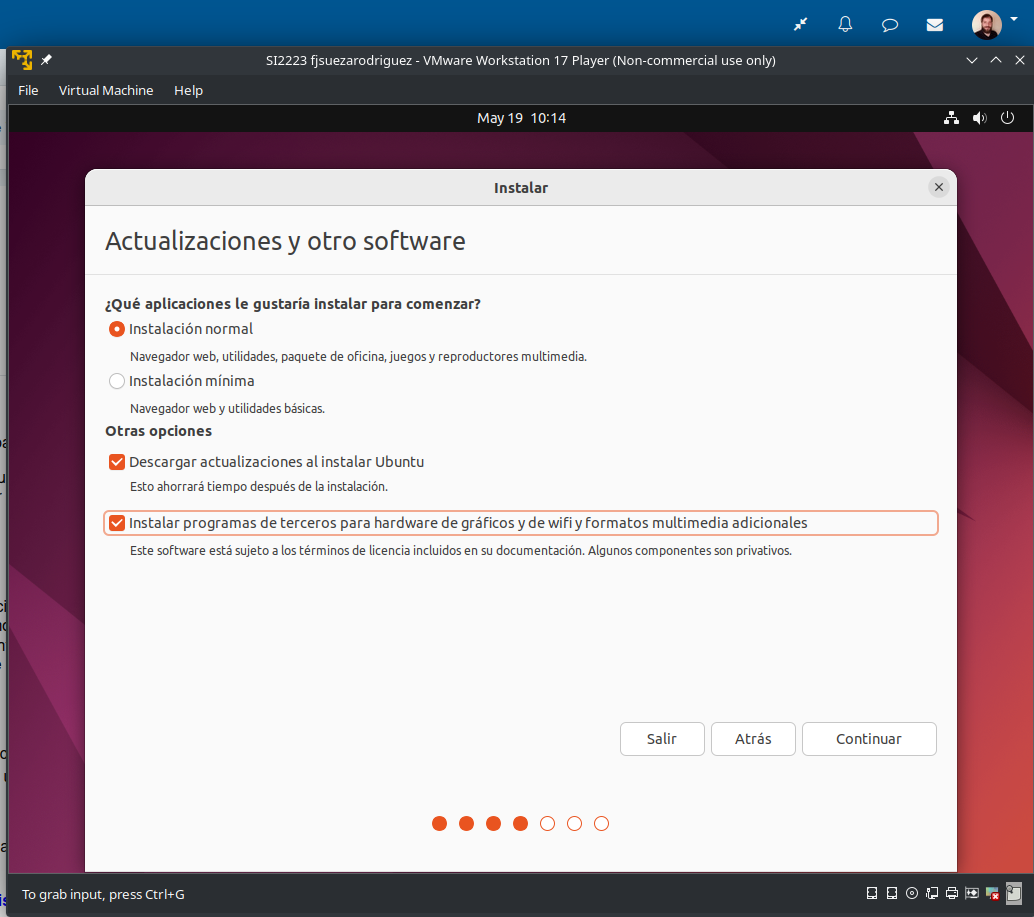
\includegraphics[scale=0.45]{ubuntu-install-5.png}
        \caption{Pantalla Actualización y Otro Software}
    \end{figure}

    \item En la siguiente pantalla, se nos permite elegir el \textbf{tipo de instalación} que queremos realizar. Aquí nos dan varias opciones que explicaremos brevemente a continuación.

    La primera opción es \textbf{Instalar Ubuntu junto a Windows Boot Manager}. Esta opción, nos dejará instalar Ubuntu junto a Windows, lo que nos permitirá elegir entre el sistema operativo que queremos iniciar durante el proceso de booteo. En este caso, se instalará GRUB junto al Gestor de Boot de Windows y el sistema se instalará en alguna partición que quede libre en el mismo disco duró donde este Windows, previo formateo con el sistema de archivo \textbf{Ext4}.

    La siguiente opción, \textbf{Borrar disco e Instalar Ubuntu}, realizará un formateo completo del disco duro e instalará Ubuntu en todo el disco duro.

    Por último, tenemos la opción \textbf{Más opciones}, Esta opción nos mostrará la tabla de particiones y nos permitirá cambiar el número de particiones, formatearlas, generar nuevas tablas de particiones, etc...

    Hemos \textbf{elegido esta última opción}, ya que vamos a \textbf{realizar 3 particiones diferentes} para la instalación de Ubuntu en el espacio libre que dejamos después de las instalación de Windows 10, que son, aproximadamente, 30 GB. Las particiones que vamos a crear y su uso serán las siguientes:

    \begin{figure}[H]
        \centering
        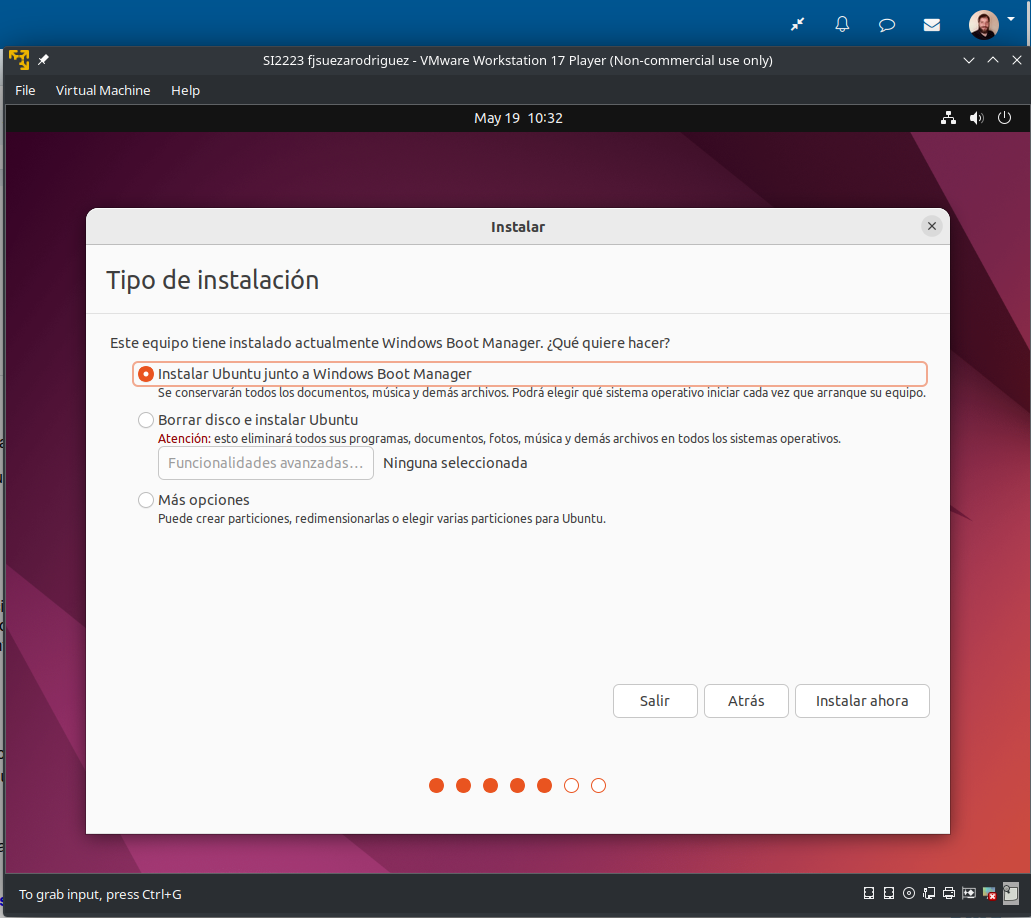
\includegraphics[scale=0.45]{ubuntu-install-6.png}
        \caption{Selección del tipo de instalación}
    \end{figure}

    \item Tras elegir la opción de instalación \textbf{Mas opciones}, se nos mostrará una ventana con información sobre la tabla de particiones que nos permitirá realiza modificaciones en ésta creando, borrando y cambiando las particiones que tiene el disco duro. En nuestro vaso, \textbf{hemos creado 3 particiones} para realizar la instalación de Ubuntu.

    En este punto no vamos a entrar más en detalles, ya que en el siguiente ejercicio hablaremos de forma más extensa sobre el particionado y como ha quedado la tabla de particiones tras la instalación, así como el uso que se le va a dar a cada una de ellas.

    \item Tras pulsar en \textbf{Instalar ahora} en la ventana de particionamiento, se nos mostrará el siguiente paso de la instalación, con una ventana donde podremos \textbf{crear el usuario por defecto}, el \textbf{nombre de equipo}, así como la contraseña de dicho usuario.

    Nosotros hemos introducido los datos pedidos en el enunciado, esto es, nuestro usuario será \textbf{fsuezarodriguez} y nuestra contraseña {admin2223}. También hemos introducido el nombre completo así como el nombre del equipo.

    Se ha marcado la opción \textbf{Iniciar sesión automática} para que no nos pida la contraseña al iniciar el sistema, aunque esto no es lo idóneo si el sistema lo van a usar varios usuarios por ejemplo, aunque no es nuestro caso.

    \begin{figure}[H]
        \centering
        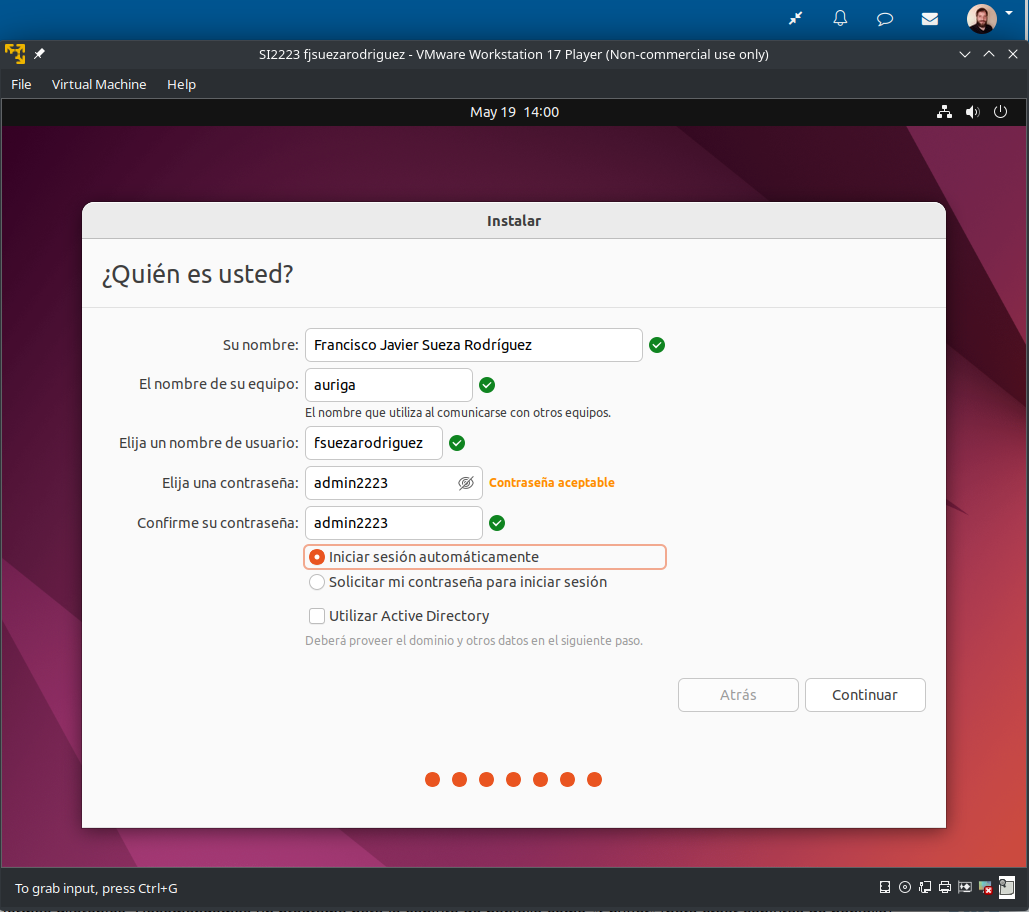
\includegraphics[scale=0.41]{ubuntu-install-8.png}
        \caption{Creación del usuario inicial y contraseña}
    \end{figure}

    \item Tras copiarse los archivos, la \textbf{instalación se habrá completado}.

    \begin{figure}[H]
        \centering
        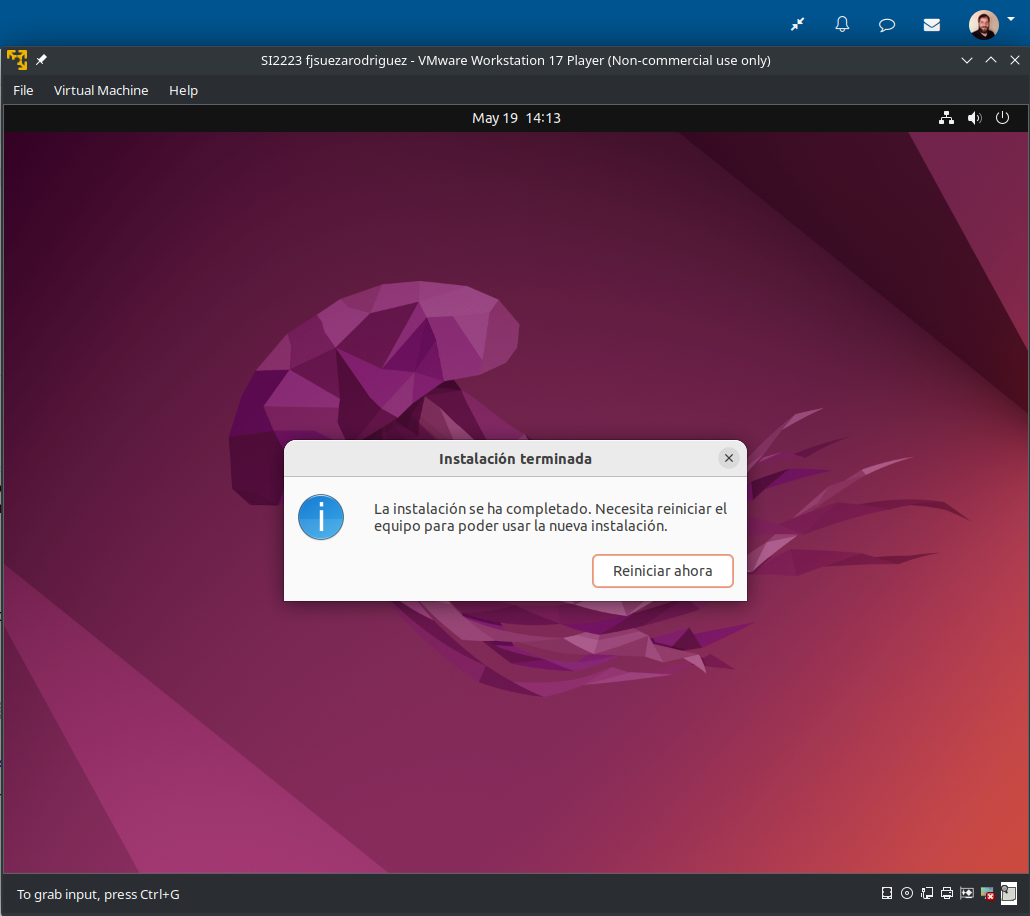
\includegraphics[scale=0.42]{ubuntu-install-7.png}
        \caption{Instalación de Ubuntu completada}
    \end{figure}
\end{enumerate}

\subsection{Ejercicio 3}

\subsubsection{Enunciado}
Muestra el esquema de particionado definitivo del disco duro tras la instalación e indica lo que contiene cada una de las particiones, incluyendo aquellas que se crearon durante las instalaciones de Windows 8.1 y Windows 10. Puedes utilizar la herramienta de gestión de particiones incluida en Ubuntu llamada "Discos".

\textbf{Capturas}:
\begin{itemize}
    \item Esquema de particionado en el que se vean todas las particiones del disco duro. Detalla el contenido de cada una de ellas.
\end{itemize}

\subsubsection{Solución}
En este ejercicio vamos a mostrar la como ha quedado la tabla de particiones en nuestra máquina virtual después de la instalación de Ubuntu, explicando los datos de cada partición. Se ha usado el programa \textbf{Discos} que incluye Ubuntu para mostrar esta información, la cual podemos ver en la siguiente captura.

\begin{figure}[H]
    \centering
    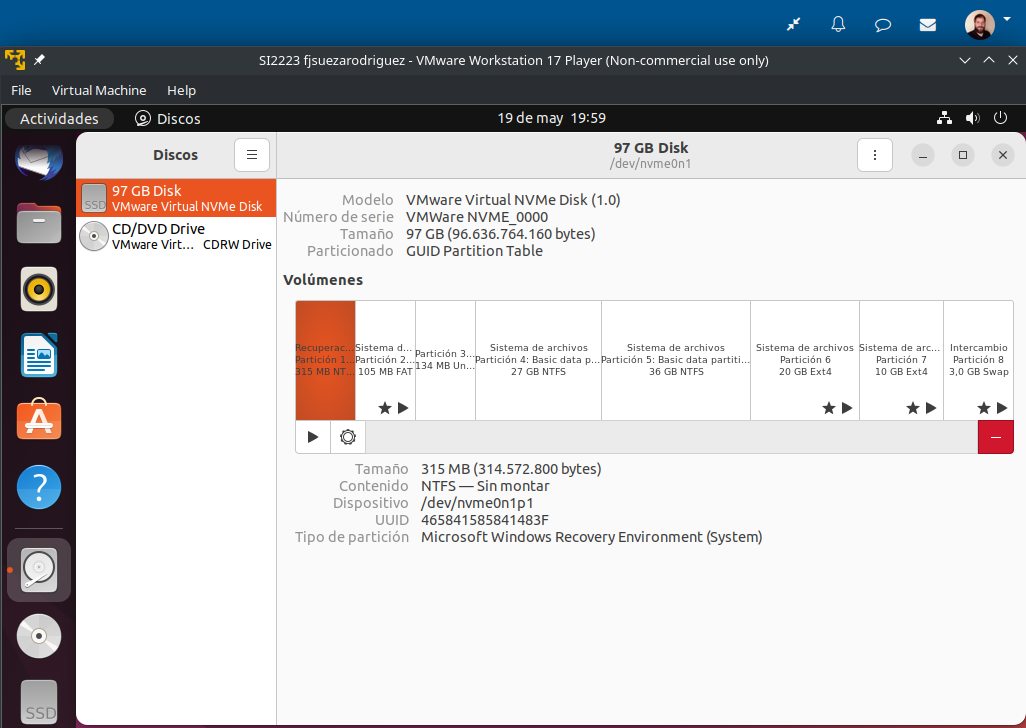
\includegraphics[scale=0.55]{particiones.png}
    \caption{Tabla de particiones desde la aplicación Discos}
\end{figure}

Como podemos ver, en la tabla de particiones hay \textbf{8 particiones}, las que pasamos a describir a continuación:

 \begin{itemize}
    \item \textbf{Partición 1}:
    \begin{itemize}
        \item \textbf{Tipo de Partición}: Primaria
        \item \textbf{Tamaño}: 315 MB
        \item \textbf{Sistemas de Archivos}: NTFS
        \item \textbf{Punto de montaje}: Ninguno
        \item \textbf{Uso}: esta es la partición Windows Recovery Environment, partición creada por el sistema Windows en su proceso de instalación y que nos sirve para recuperar el sistema en caso de que haya algún fallo.
    \end{itemize}

        \item \textbf{Partición 2}:
        \begin{itemize}
            \item \textbf{Tipo de Partición}: Primaria
            \item \textbf{Tamaño}: 105 MB
            \item \textbf{Sistemas de Archivos}: FAT
            \item \textbf{Punto de montaje}: /boot/efi
            \item \textbf{Uso}: partición del sistema de arranque EFI, independiente del sistema operativo y donde se almacenan los diferentes cargadores de los sistemas operativos.
        \end{itemize}

    \item \textbf{Partición 3}:
    \begin{itemize}
        \item \textbf{Tipo de Partición}: Primaria
        \item \textbf{Tamaño}: 134 MB
        \item \textbf{Sistemas de Archivos}: ?
        \item \textbf{Punto de montaje}: Ninguno
        \item \textbf{Uso}: esta es la partición MSR, partición reservada por Microsoft y que crean los sistemas Windows, desde Windows 7, durante el proceso de instalación
        para uso posterior del sistema operativo y almacenar ciertos archivos de arranque.
    \end{itemize}

    \item \textbf{Partición 4}:
    \begin{itemize}
        \item \textbf{Tipo de Partición}: Primaria
        \item \textbf{Tamaño}: 27 GB
        \item \textbf{Sistemas de Archivos}: NTFS
        \item \textbf{Punto de montaje}: Sin montar
        \item \textbf{Uso}: partición de datos básica de Windows donde se ha realizado la instalación de Windows 8.1.
    \end{itemize}

    \item \textbf{Partición 5}:
    \begin{itemize}
        \item \textbf{Tipo de Partición}: Primaria
        \item \textbf{Tamaño}: 36 GB
        \item \textbf{Sistemas de Archivos}: NTFS
        \item \textbf{Punto de montaje}: Sin montar
        \item \textbf{Uso}: partición de datos básica de Windows donde se ha realizado la instalación de Windows 10.
    \end{itemize}

    \item \textbf{Partición 6}:
    \begin{itemize}
        \item \textbf{Tipo de Partición}: Primaria
        \item \textbf{Tamaño}: 20 GB
        \item \textbf{Sistemas de Archivos}: Ext4
        \item \textbf{Punto de montaje}: / (sistema raíz)
        \item \textbf{Uso}: esta partición la vamos a emplear para instalar el sistema operativo. Será donde irán todas las aplicaciones instaladas, tanto durante el proceso de instalación como las que instalemos en un futuro.
    \end{itemize}


    \item \textbf{Partición 7}:
    \begin{itemize}
        \item \textbf{Tipo de Partición}: Primaria
        \item \textbf{Tamaño}: 10 GB
        \item \textbf{Sistemas de Archivos}: Ext4
        \item \textbf{Punto de montaje}: /home
        \item \textbf{Uso}: en esta partición se almacenarán los directorios personales de los usuarios. Es una buena práctica poner estos directorios en una partición independiente, ya que si en un futuro tuviéramos que reinstalar el sistema, podríamos dejar esta partición sin tocar con lo que todos los archivos de los diferentes usuarios no se perderían.
    \end{itemize}

    \item \textbf{Partición 8}:
    \begin{itemize}
        \item \textbf{Tipo de Partición}: Swap (área de intercambio)
        \item \textbf{Tamaño}: 3 GB
        \item \textbf{Sistemas de Archivos}: Linux Swap Filesystem
        \item \textbf{Punto de montaje}: Ninguno
        \item \textbf{Uso}: esta partición se usará como área de intercambio, para almacenar operaciones que deberían estar en la memoria RAM pero no están ahora mismo en estado de ejecución, proporcionando una RAM virtual. En nuestro caso es de especial utilidad, ya que la memoria que tenemos asignada a la Máquina Virtual es poca.
    \end{itemize}
\end{itemize}

\subsection{Actividad 4}

\subsubsection{Enunciado}
Selecciona el mejor servidor de descarga de repositorios atendiendo a tu ubicación y, a continuación, actualiza los repositorios. Una vez hecho esto, actualiza el sistema utilizando:

\begin{enumerate}
    \item El terminal
    \item La herramienta "Actualización de software".
\end{enumerate}

\textbf{Capturas}
\begin{itemize}
    \item Ventana donde se elije el mejor servidor de descarga de repositorios atendiendo a tu ubicación (indica textualmente cómo se accede a dicha ventana).
    \item Comando/s usado/s en el terminal y resultado del mismo/s, para la actualización de repositorios y para la actualización del sistema.
    \item Ventana donde se realiza la actualización del sistema (indica textualmente cómo se accede a dicha ventana) y resultado final.
\end{itemize}

\subsection{Solución}
En este ejercicio vamos a cambiar el servidor de descarga de repositorios, eligiendo el más cercado a nuestra ubicación lo que hará que las descargas sean más rápidas y tengan menos latencia. Para llevar esto a cabo, vamos a usar la aplicación \textbf{Software y Actualizaciones} de Ubuntu, a la que podemos acceder pulsando en el botón \textbf{Mostrar Aplicaciones} de la barra latera y introduciendo \textbf{Software y Actualizaciones} en el formulario de búsqueda.

Una vez se abra la aplicación, veremos la opción \textbf{Descargar desde} con un menú desplegable donde podremos seleccionar el \textbf{Servidor para España}, como podemos ver en la siguiente captura.

\begin{figure}[H]
    \centering
    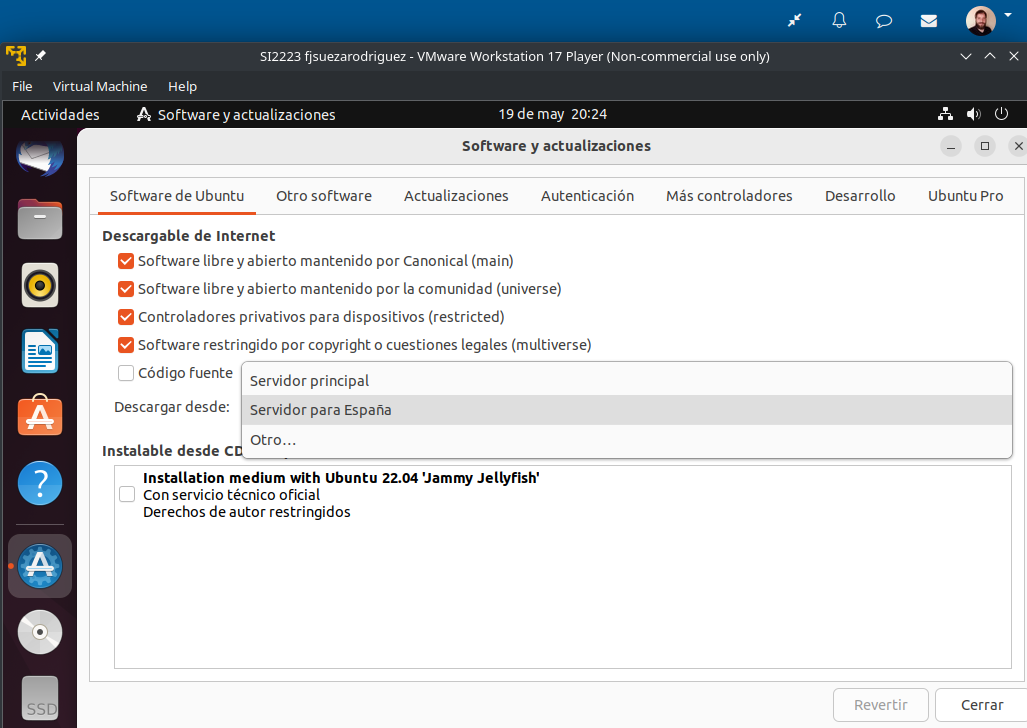
\includegraphics[scale=0.50]{repos-1.png}
    \caption{Software y Actualizaciones en Ubuntu}
\end{figure}

A continuación, vamos a \textbf{actualizar los repositorios} con el servidor seleccionado, lo cual vamos a hacer de dos formas diferentes, usando en primer lugar \textbf{APT} para realizar la actualización de los repositorios y del sistema desde \textbf{la termina} y después usando herramienta gráfica \textbf{Actualización de Software}

\begin{enumerate}
    \item \textbf{Terminal}: para actualizar los repositorios desde la terminal, debemos usar el comando \textbf{apt-get update}, mientras que para actualizar el sistema usaremos \textbf{apt-get dist-upgrade}, ambos comandos precedidos del comando \textbf{sudo}, ya que necesitamos privilegios de administrados.

    \begin{figure}[H]
        \centering
        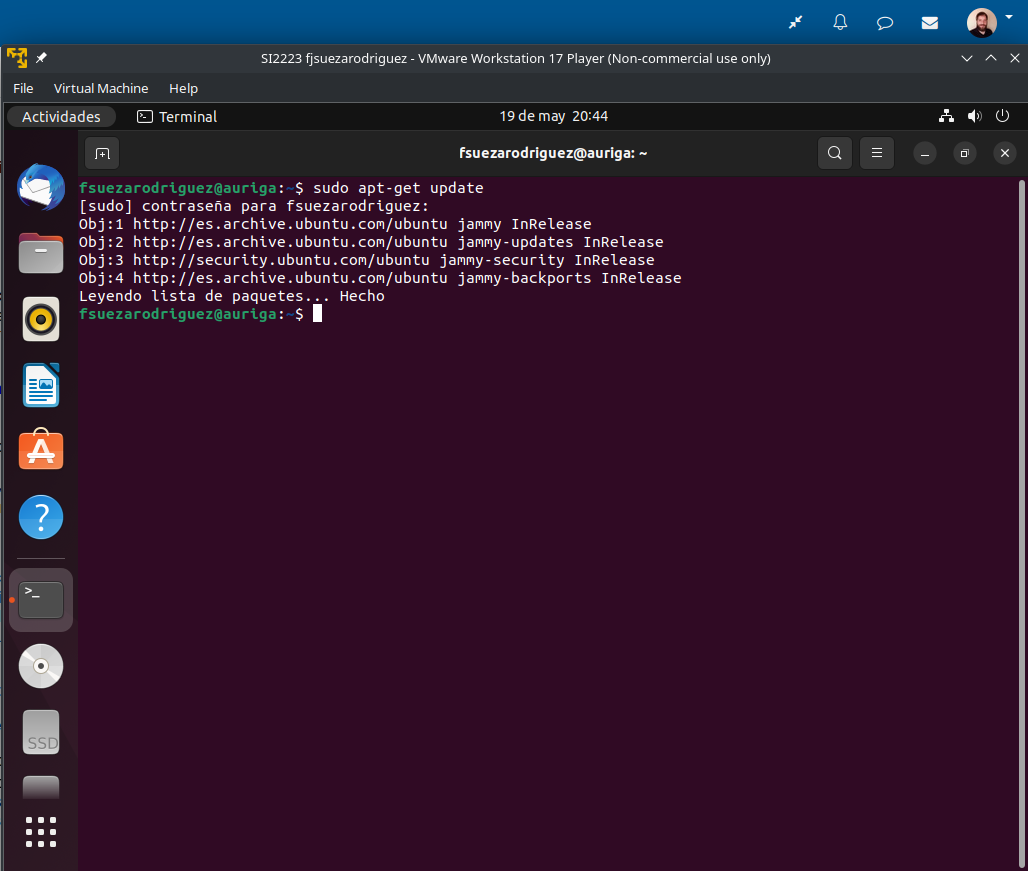
\includegraphics[scale=0.44]{repos-2.png}
        \caption{Actualización de repositorios con apt-get}
    \end{figure}

    \begin{figure}[H]
        \centering
        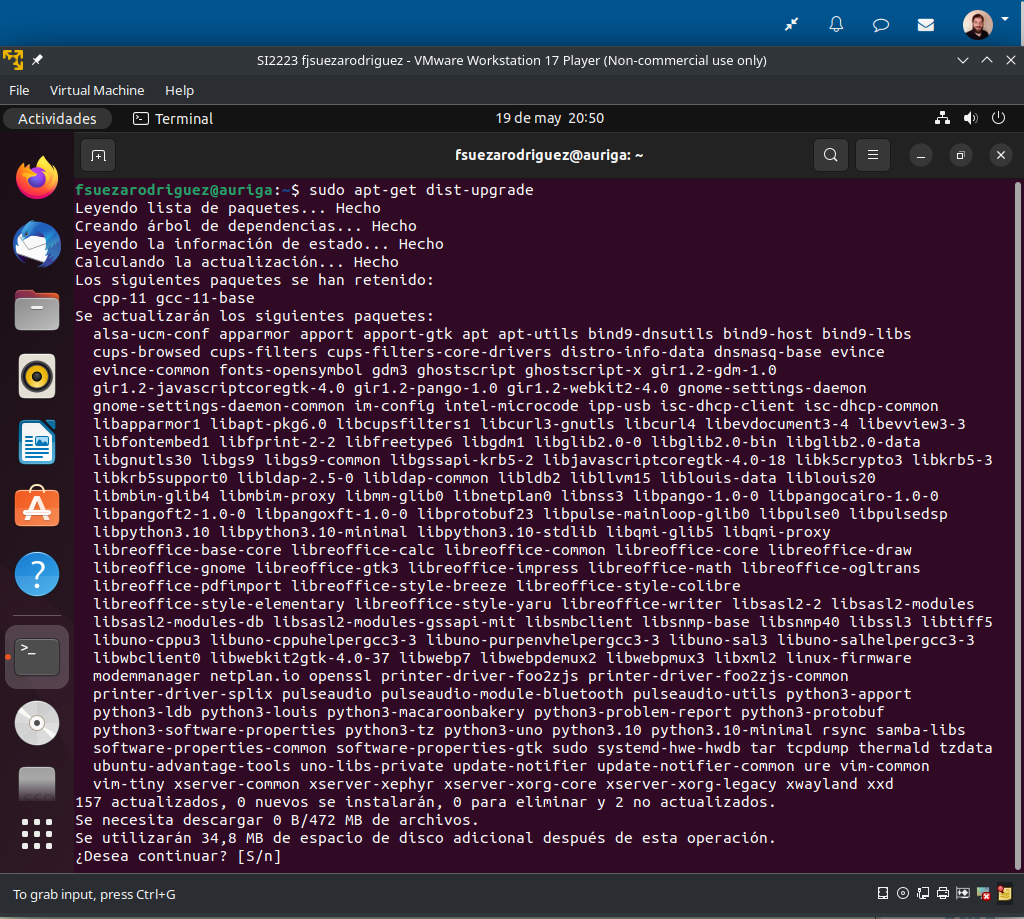
\includegraphics[scale=0.44]{repos-3.png}
        \caption{Actualización del sistema con apt-get}
    \end{figure}

    Como vemos en la última captura, cuando ejecutemos \textbf{apt-get dist-upgrade} se nos mostrarán todos los paquetes que se van a actualizar, pidiéndonos la confirmación de la actualización. Tras introducir la letra \textbf{S} para confirmar, la actualización de los paquetes dará comienzo.

    Una vez que haya finalizado, se nos mostrará la información en la terminal, como podemos ver en la siguiente captura.

    \begin{figure}[H]
        \centering
        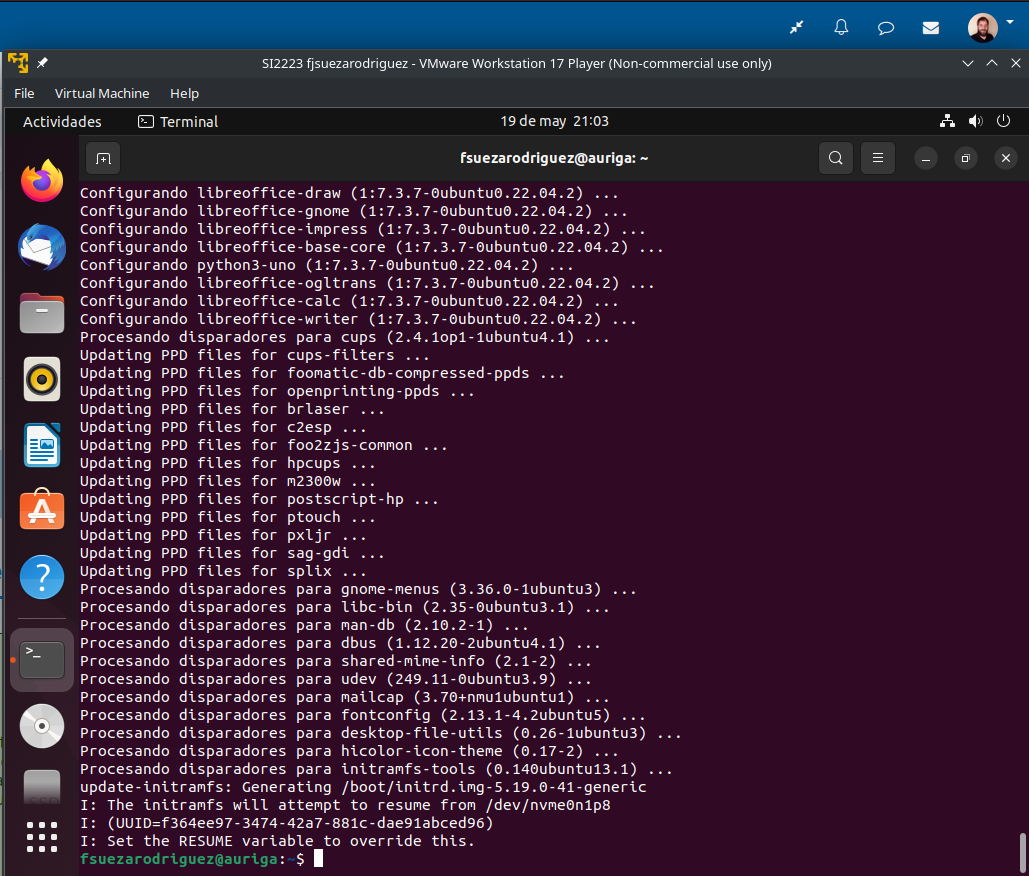
\includegraphics[scale=0.44]{repos-4.png}
        \caption{Actualización del sistema finalizada}
    \end{figure}

    \item La siguiente manera de actualizar tanto los repositorios como el sistema es empleando la herramienta gráfica que proporciona Gnome llamada \textbf{Actualización de Software}, a la cual podemos acceder pulsando en el botón \textbf{Mostrar aplicaciones} de la barra lateral e introduciendo el nombre en la caja de búsqueda. Una vez que pulsemos en su icono, la aplicación comenzarán a buscar actualizaciones de forma automáticamente.

    \begin{figure}[H]
        \centering
        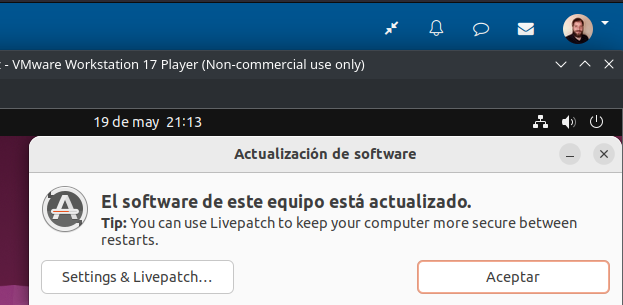
\includegraphics[scale=0.55]{repos-5.png}
        \caption{Aplicación Actualización de Software en Ubuntu}
    \end{figure}

    En nuestro caso, como hemos usado previamente el comando \textbf{apt-get dist-upgrade}, en sistema esta actualizado, como nos indica la aplicación y podemos ver en la anterior captura.
\end{enumerate}

\subsection{Actividad 5}

\subsubsection{Enunciado}
Instala y desinstala la aplicación que prefieras de dos formas diferentes. Recomendamos un programa para la captura de pantalla como "Shutter" (para crear capturas de pantalla). Consulta el apartado 7 de la unidad para elegir el método:

\begin{itemize}
    \item Utilizando el terminal (con los comandos apt-get, apt, aptitude o snap).
    \item De cualquier otra de las formas que se indican en la unidad (Synaptic,  Ubuntu Software, ...).
\end{itemize}

\textbf{Capturas}:
\begin{itemize}
    \item Comando usado para la instalación de la aplicación por terminal, mostrando el resultado del mismo. Si fuera necesario, comando para añadir el repositorio oficial del paquete.
    \item Comando usado para la desinstalación de la aplicación por terminal, mostrando el resultado del mismo.
    \item Ventana donde se solicita la instalación de la aplicación (indica textualmente cómo se accede a dicha ventana) y captura final mostrando que se completó con éxito.
    \item Ventana donde se solicita la desinstalación de la aplicación (indica textualmente cómo se accede a dicha ventana) y captura final mostrando que se completó con éxito.
\end{itemize}

\subsubsection{Solución}
En este ejercicio vamos a realizar la instalación y desinstalación de una aplicación, en concreto al aplicación \textbf{nmap}, una utilidad de red para el análisis de redes y la auditoría de seguridad.

Para realizar la instalación y desinstalación de la aplicación vamos a usar dos métodos, por un lado, vamos a realizar la instalación desde la termina usando el comando \textbf{apt-get}, por otro, realizaremos el mismo proceso usando la aplicación gráfica \textbf{Ubuntu Software}.

\begin{itemize}
    \item \textbf{Instalación/Desinstalación usando apt-get}: En primer lugar vamos a realizar la \textbf{instalación de nmap usando apt-get}. Para realizar la instalación, abrimos una terminal e introducimos el comando \textbf{apt-get install nmap}. Hay que tener en cuenta, que necesitamos tener privilegios de root para instalar paquetes, por lo que o bien deberemos estar loggeados como root o usar el comando \textbf{sudo} delante del apt-get. En la figura 2.17 podemos ver el resultado de la ejecución de este comando.

    Una vez que los tenemos instalado, vamos a proceder a realizar \textbf{la desinstalación}. Para hacerlo, vamos a usar el comando \textbf{apt-get purge}. Podríamos usar también el comando \textbf{apt-get remove}, ya que hacen básicamente lo mismo, pero con la opción \textbf{purge} de apt-get, además de eliminar los paquetes, también se eliminan los archivos de configuración asociados a dichos paquetes, haciendo una \textbf{limpieza más profunda}, por decirlo así.
    El resultado de este comando lo podemos ver en la figura 2.18 de la siguiente página.


\begin{figure}[H]
    \centering
    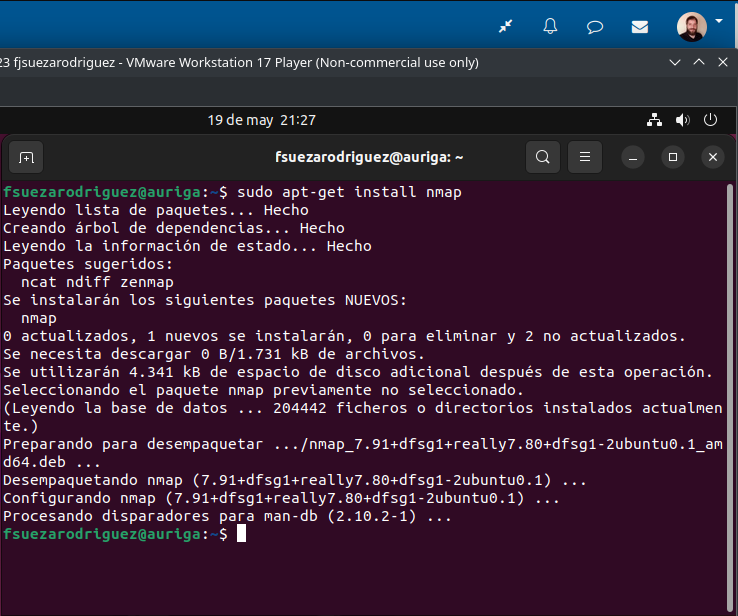
\includegraphics[scale=0.60]{install-1.png}
    \caption{Instalación de nmap con apt-get}
\end{figure}

\begin{figure}[H]
    \centering
    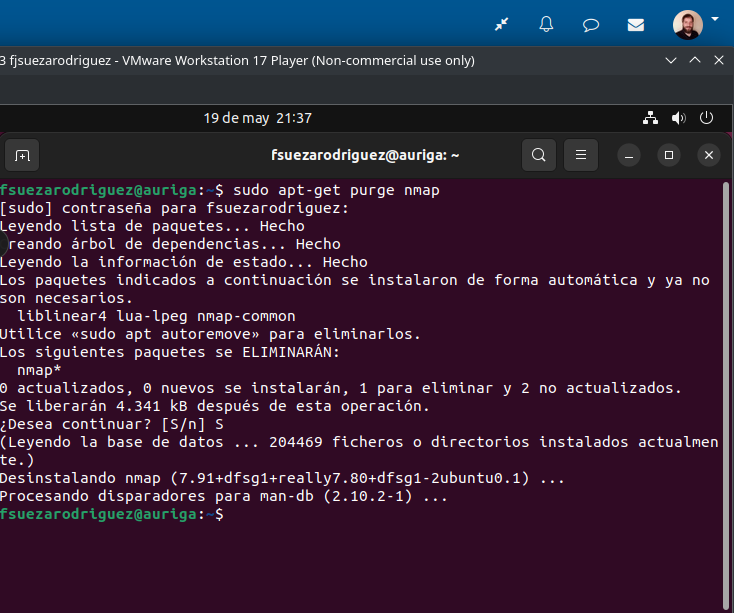
\includegraphics[scale=0.60]{install-2.png}
    \caption{Desinstalación de nmap con apt-get}
\end{figure}

    \item \textbf{Instalación/Desinstalación usando Ubuntu Software}: para iniciar la aplicación \textbf{Ubuntu Software}, pulsamos en su icono en la barra lateral del escritorio. Una vez pulsado (es un icono naranja con una A), se nos abrirá la aplicación con la pestaña \textbf{Explorar} seleccionada. A la izquierda de esta pestaña, pulsamos en el \textbf{icono con forma de lupa} que nos permitirá buscar la aplicación que queremos instalar.

    Una vez que pinchemos en el icono de la aplicación que queremos instalar, en nuestro caso, nmap, se nos abrirá una nueva ventana donde podremos ver información de la aplicación. Pulsamos en el botón \textbf{instalar}, y tras solicitarnos la contraseña de root, el proceso de instalación comenzará.

    \begin{figure}[H]
        \centering
        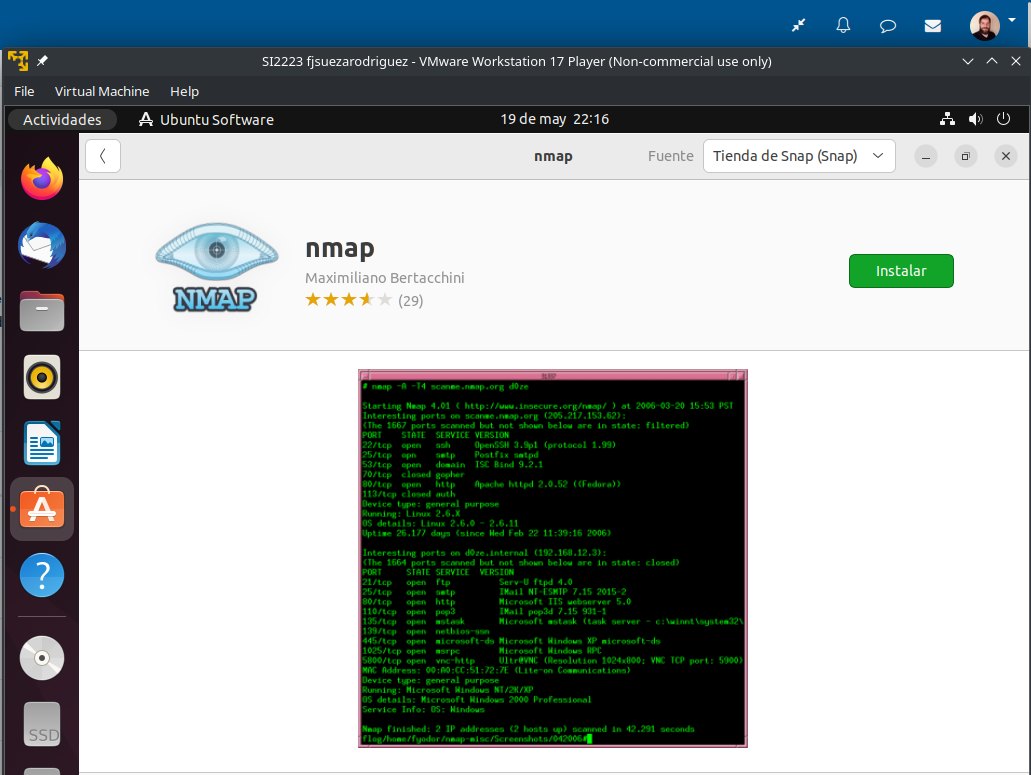
\includegraphics[scale=0.35]{install-3.png}
        \caption{Inicio de instalación de nmap desde Ubuntu Software}
    \end{figure}

    Tras la instalación, el botón de \textbf{instalar} cambiará a un icono rojo con un cubo de basura, que nos permite desinstalar la aplicación, indicando que se instalación se ha realizado correctamente.

   \begin{figure}[H]
        \centering
        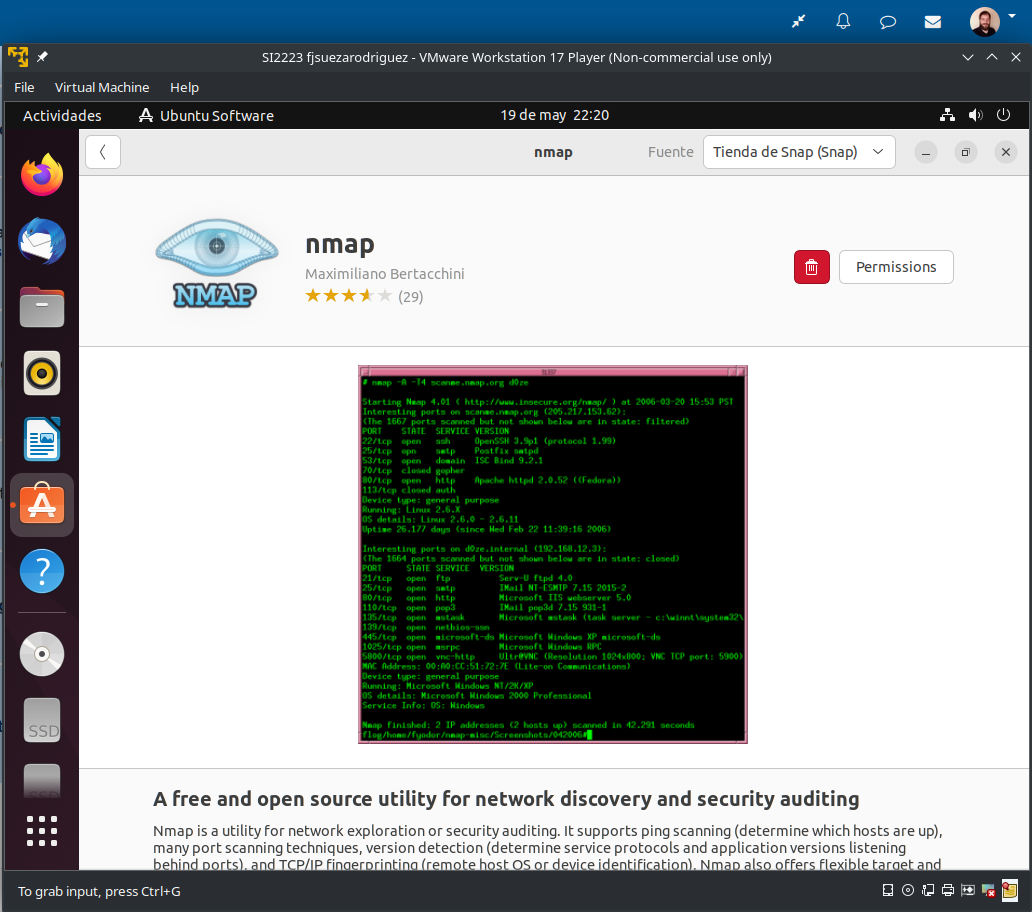
\includegraphics[scale=0.35]{install-4.png}
        \caption{Instalación completada de nmap desde Ubuntu Software}
    \end{figure}

    Para realizar la \textbf{desinstalación}, solo hay que pulsar en el \textbf{botón rojo}, que podemos ver en al captura anterior, y tras pedirnos la confirmación, la desinstalación se realizará correctamente.

   \begin{figure}[H]
        \centering
        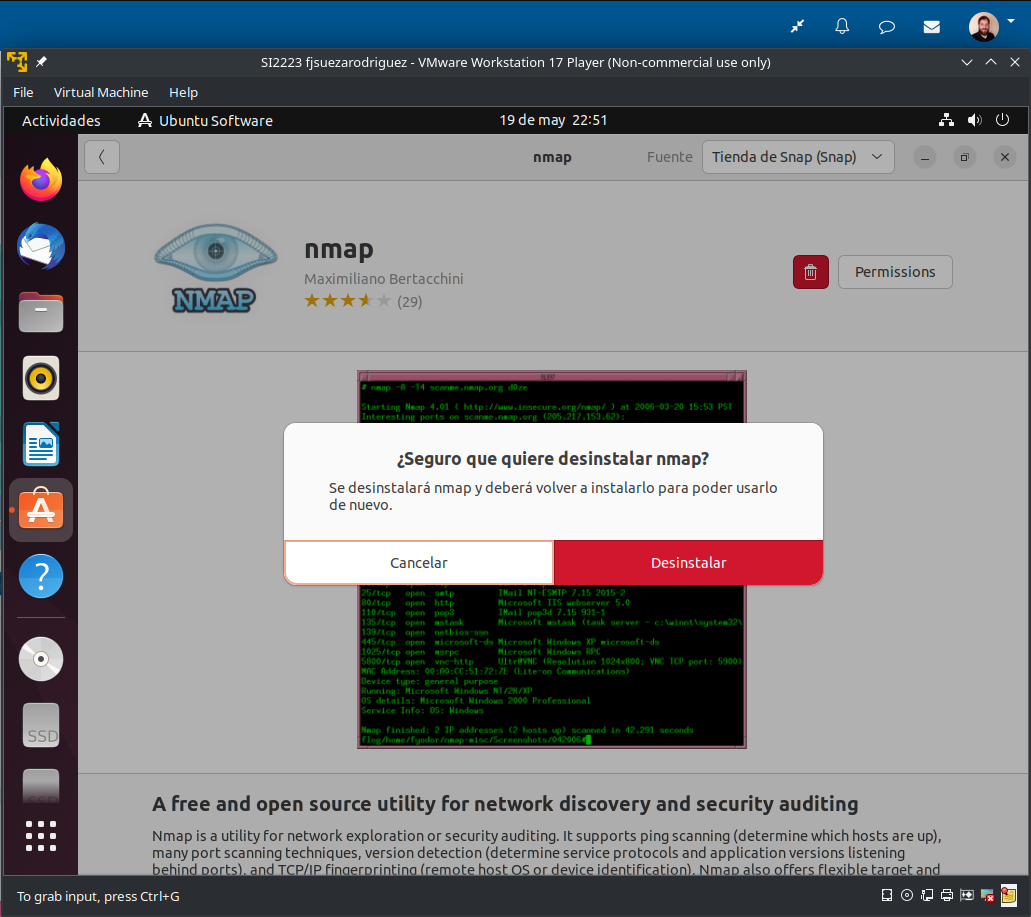
\includegraphics[scale=0.45]{install-5.png}
        \caption{Desinstalación de nmap desde Ubuntu Software}
    \end{figure}
\end{itemize}
% Bibliography

%\newpage
%\bibliography{citas}
%\bibliographystyle{unsrt}

\end{document}